% !TEX root =  ../main.tex


\begin{figure*}[t]
	\centering
	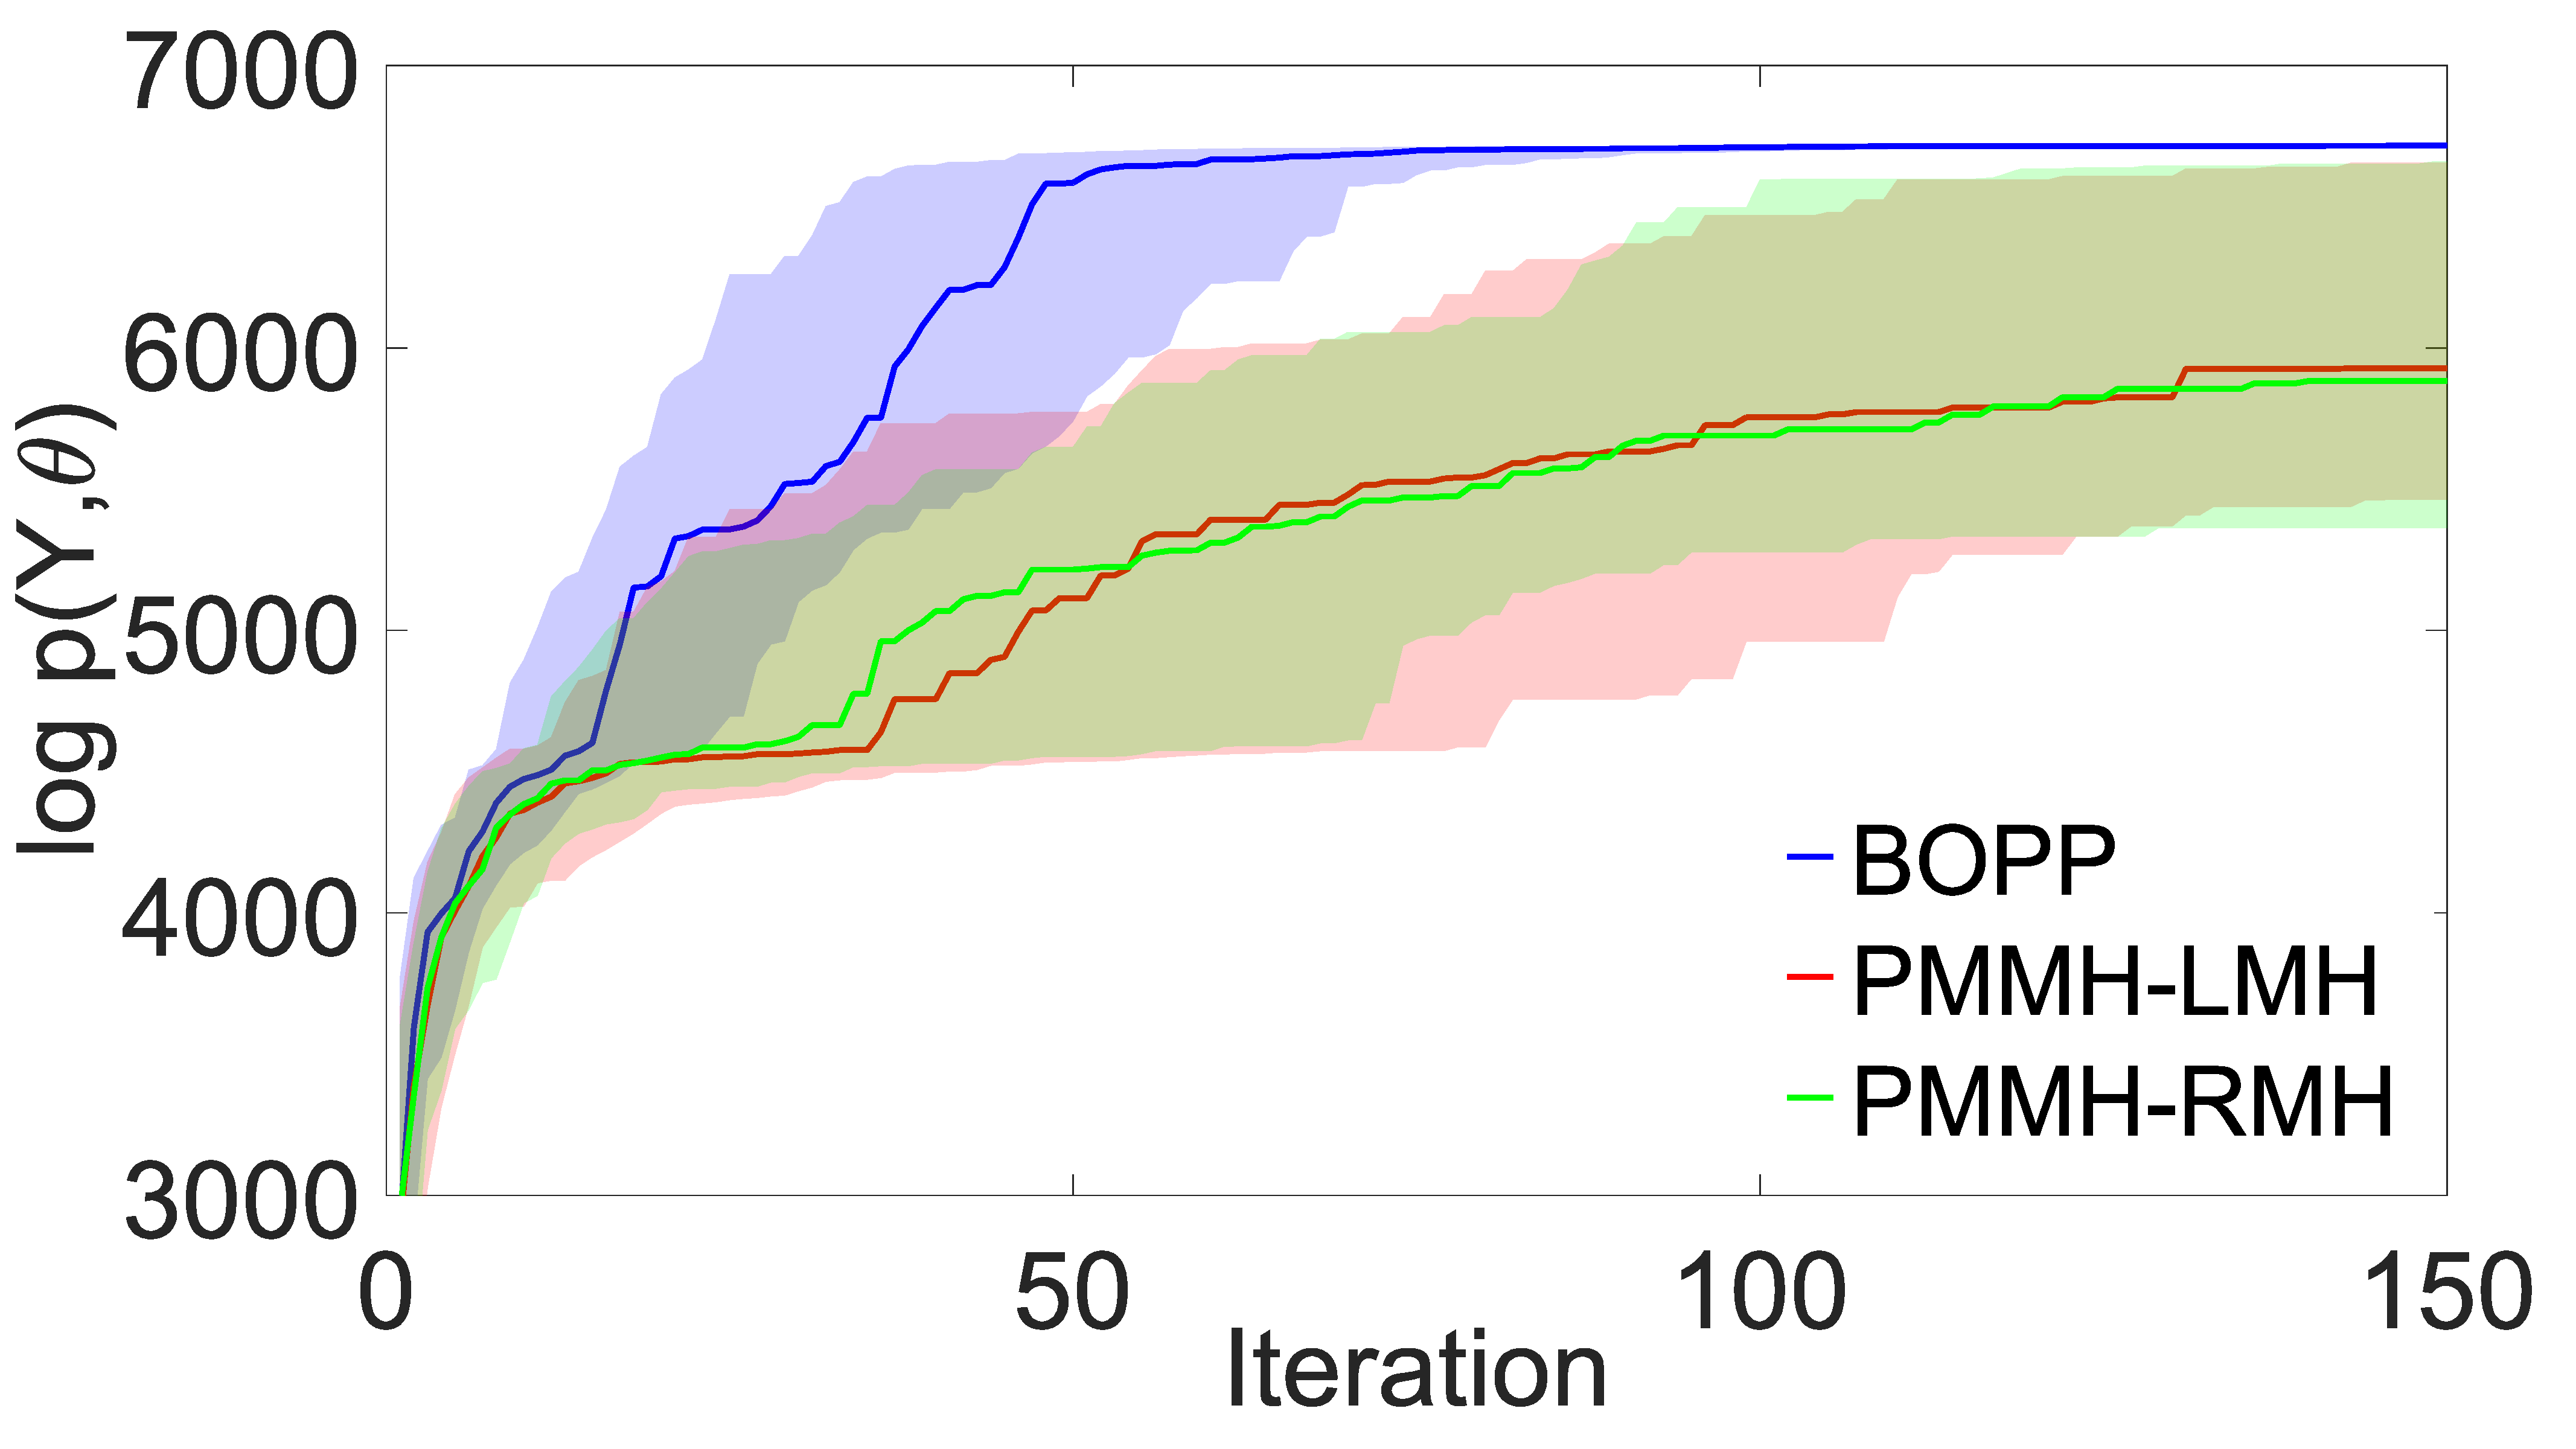
\includegraphics[width=2.72in]{chaos/chaos_ml.pdf}
	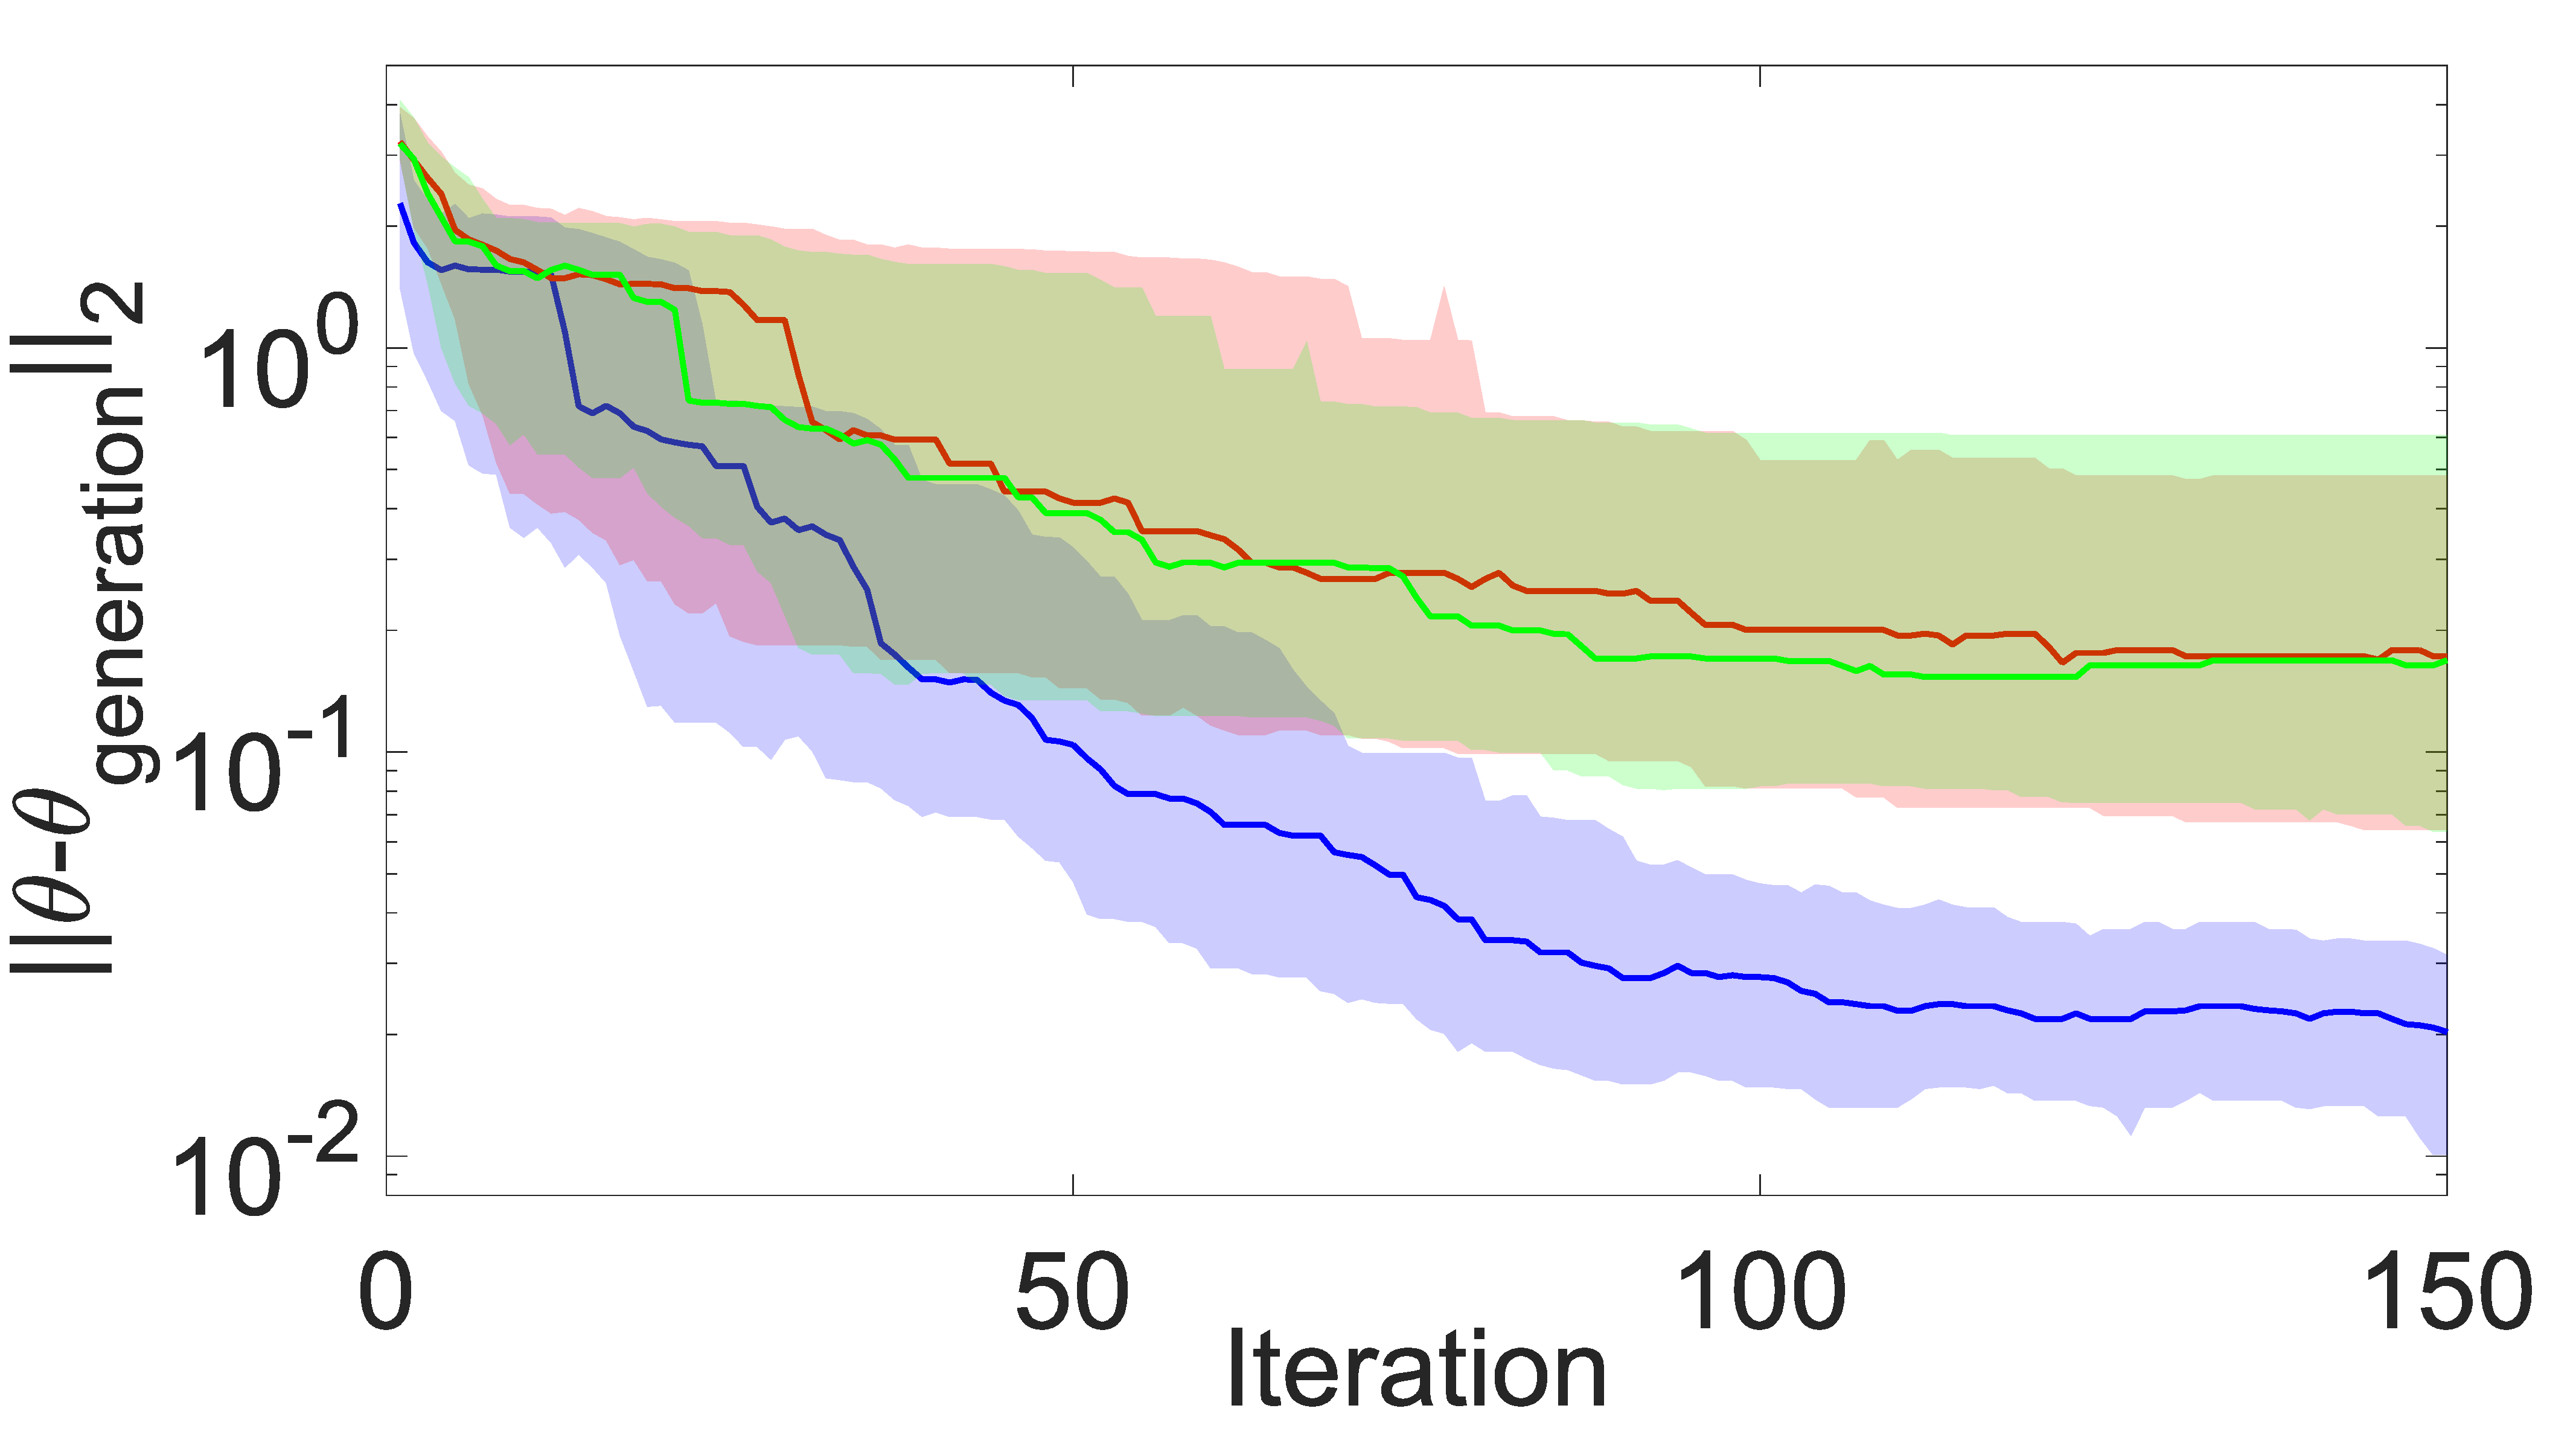
\includegraphics[width=2.72in]{chaos/chaos_distance.pdf}
	\caption{Convergence for transition dynamics parameters of the pickover attractor in terms of the cumulative best $\log p\left(Y,\theta\right)$ (\emph{left}) and distance to the ``true" $\theta$ used in generating the data (\emph{right}). Solid line shows median over 100 runs, whilst the shaded region the 25/75\% quantiles.  \label{fig:chaos}
		\vspace{6pt}}
\end{figure*}

\begin{figure}[t]
	\centering
	\begin{subfigure}[t]{0.24\textwidth}
		\centering
		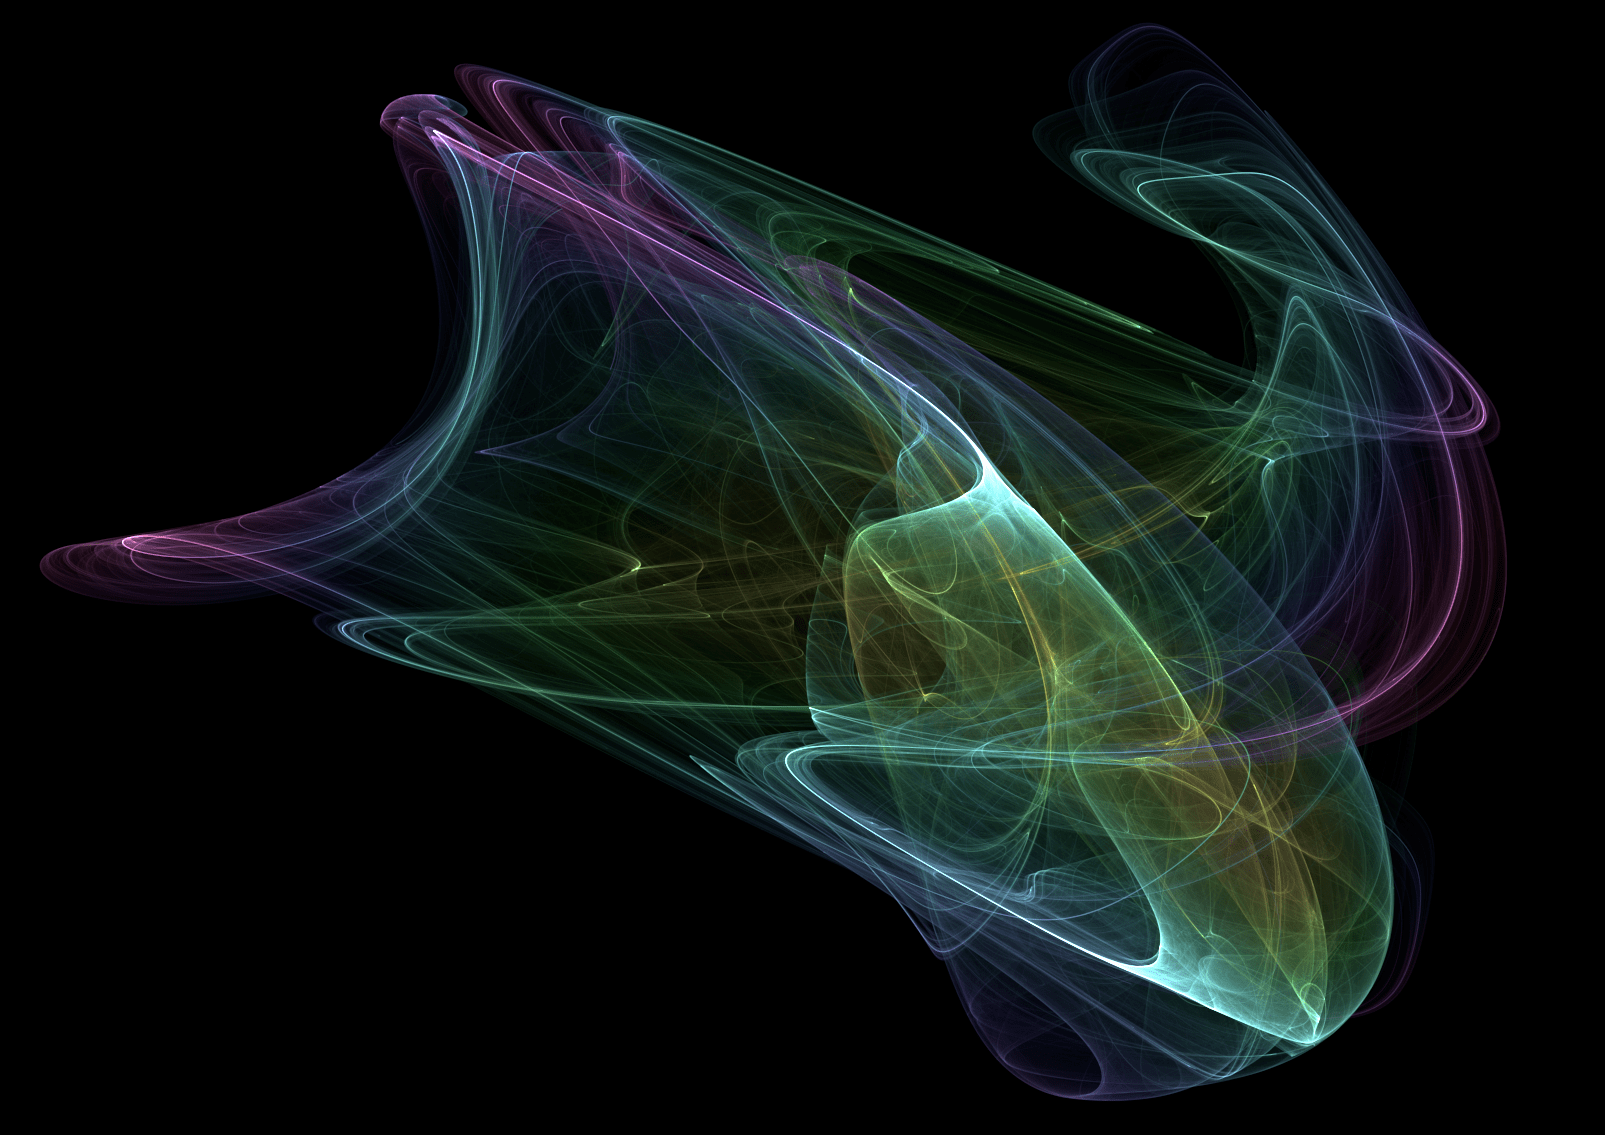
\includegraphics[height=3.2cm,width=3.7cm]{chaos/compressed/first_iter_alt.png}
		\caption{1 iteration}
	\end{subfigure}
	\begin{subfigure}[t]{0.24\textwidth}
		\centering
		\tiny
		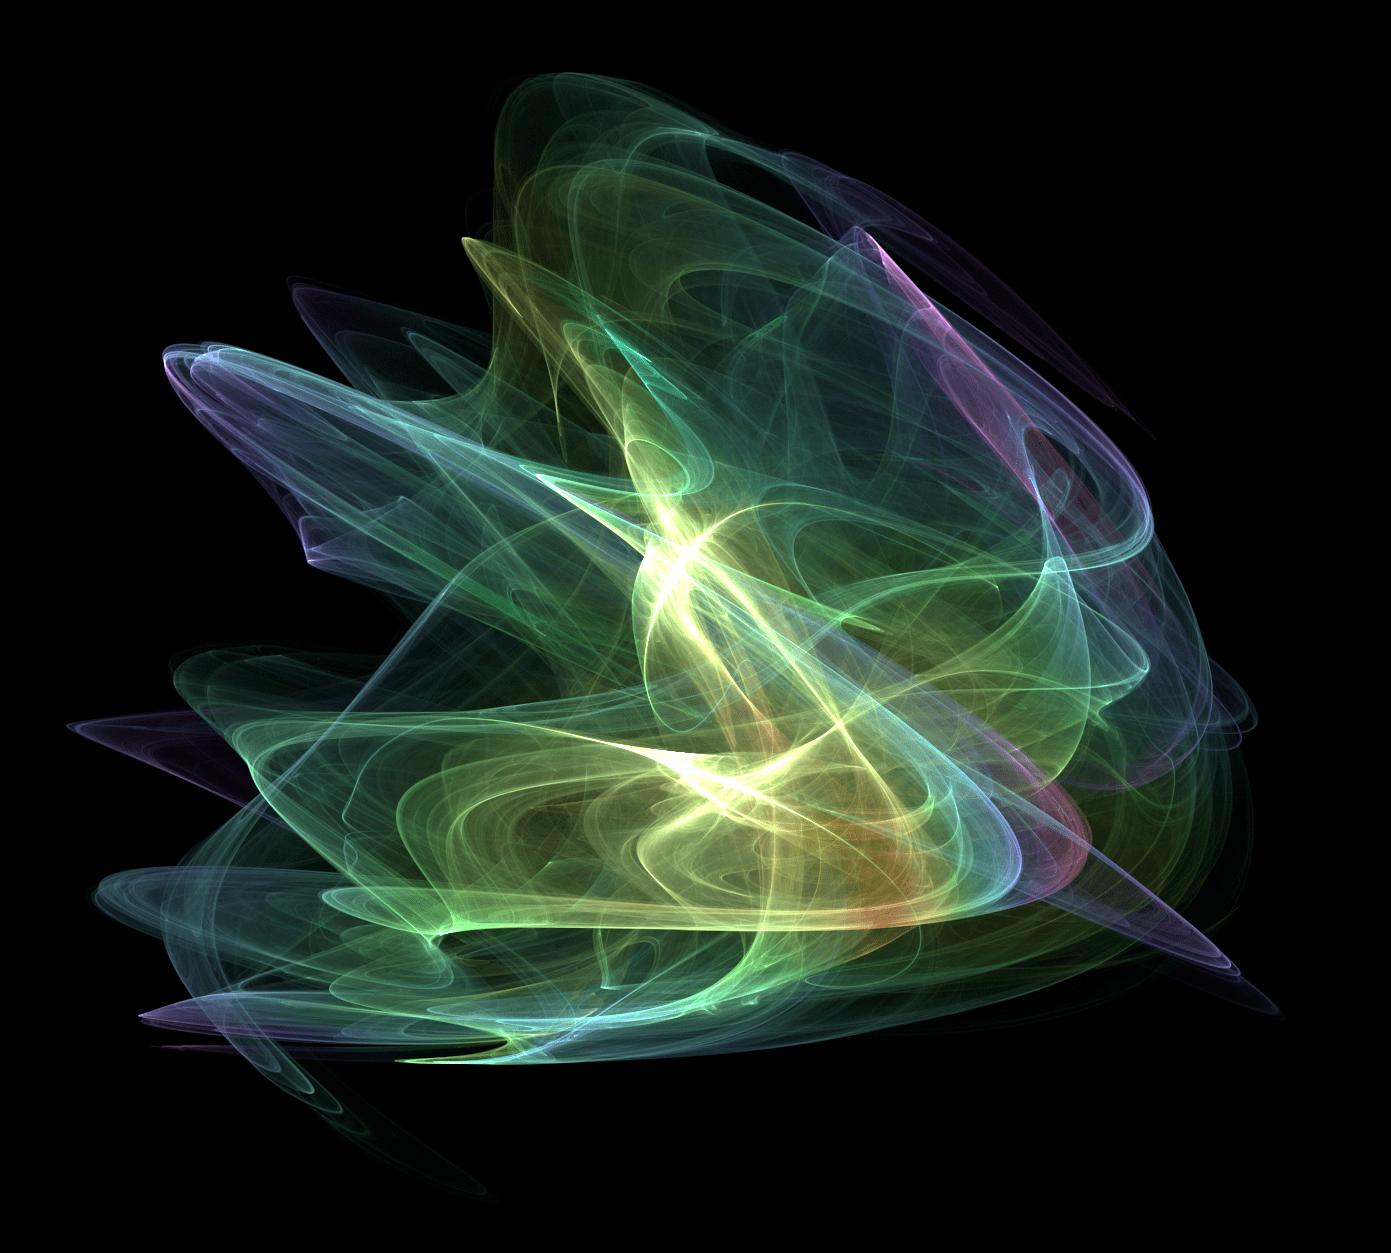
\includegraphics[height=3.2cm,width=3.7cm]{chaos/compressed/20_iter_alt.png}
		\caption{20 iterations}
	\end{subfigure}
	\begin{subfigure}[t]{0.24\textwidth}
		\centering
		\tiny
		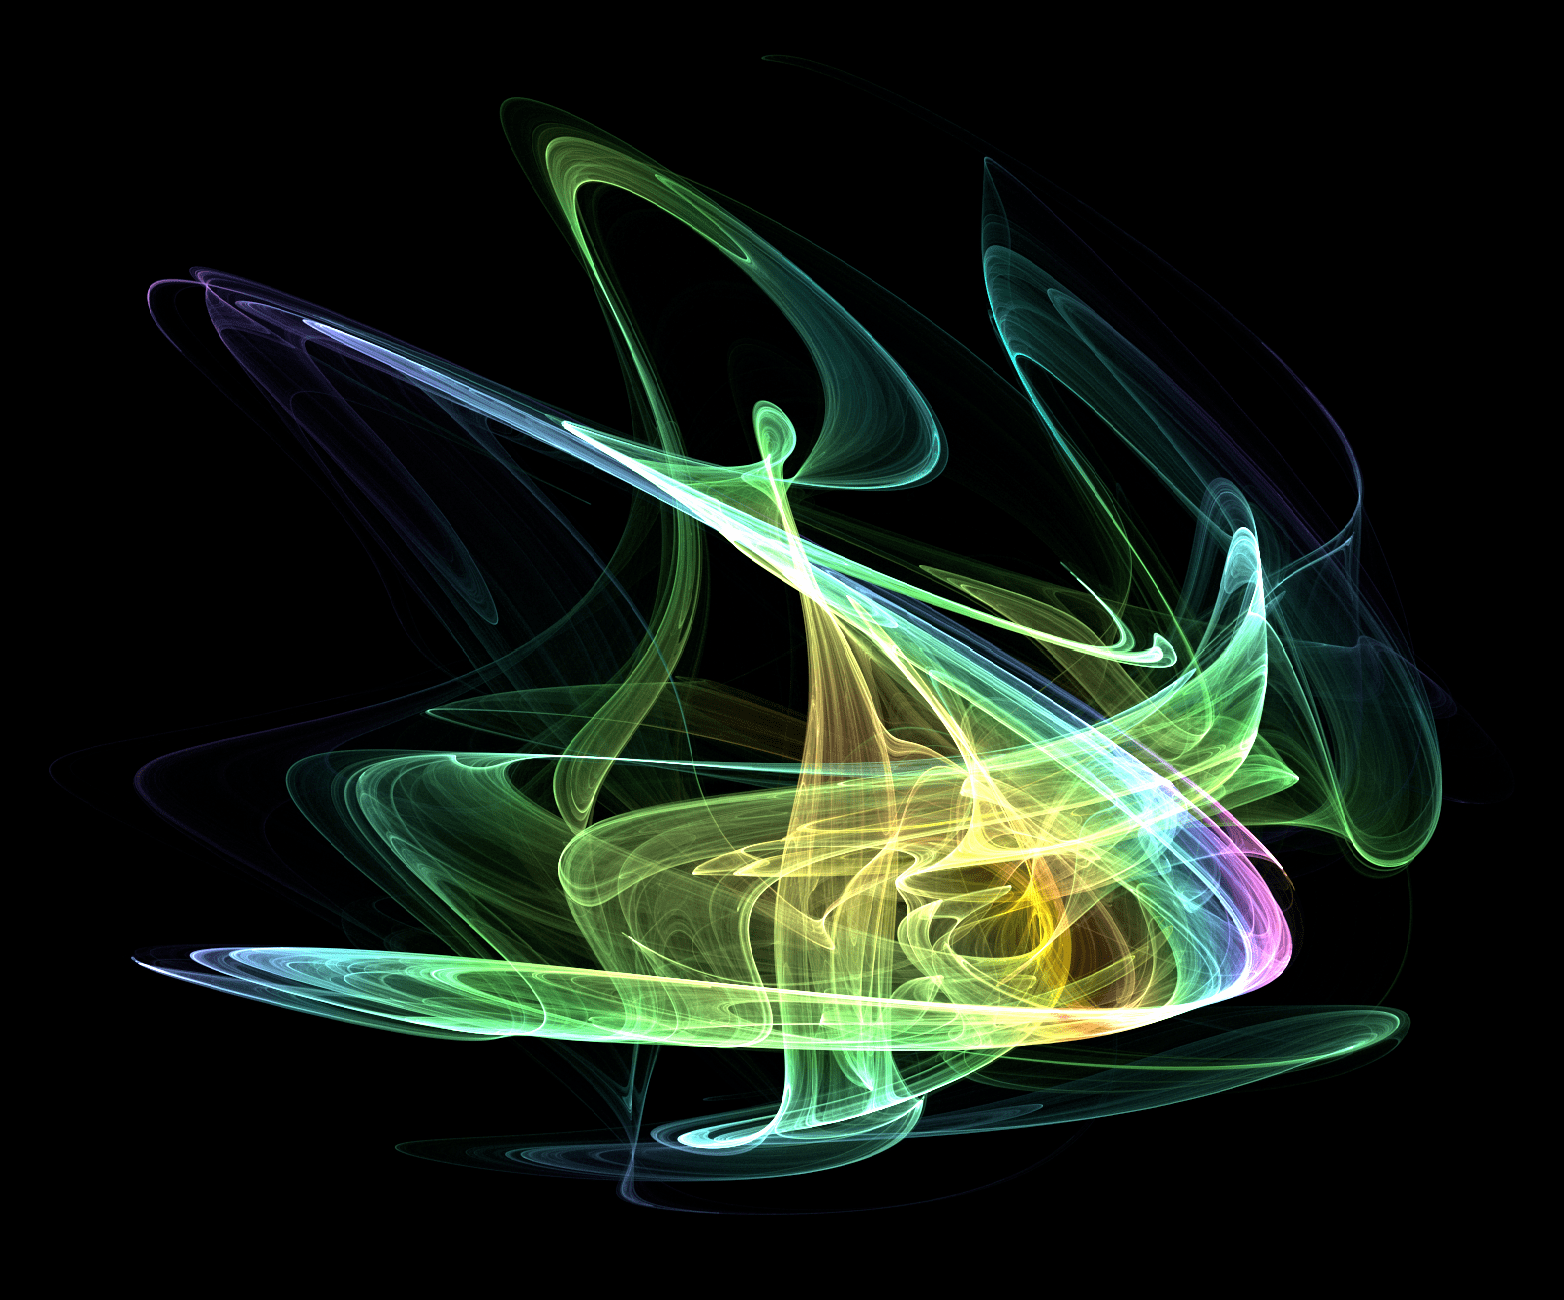
\includegraphics[height=3.2cm,width=3.7cm]{chaos/compressed/100_iter_altj.png}
		\caption{100 iterations}
	\end{subfigure}
	\begin{subfigure}[t]{0.24\textwidth}
		\centering
		\tiny
		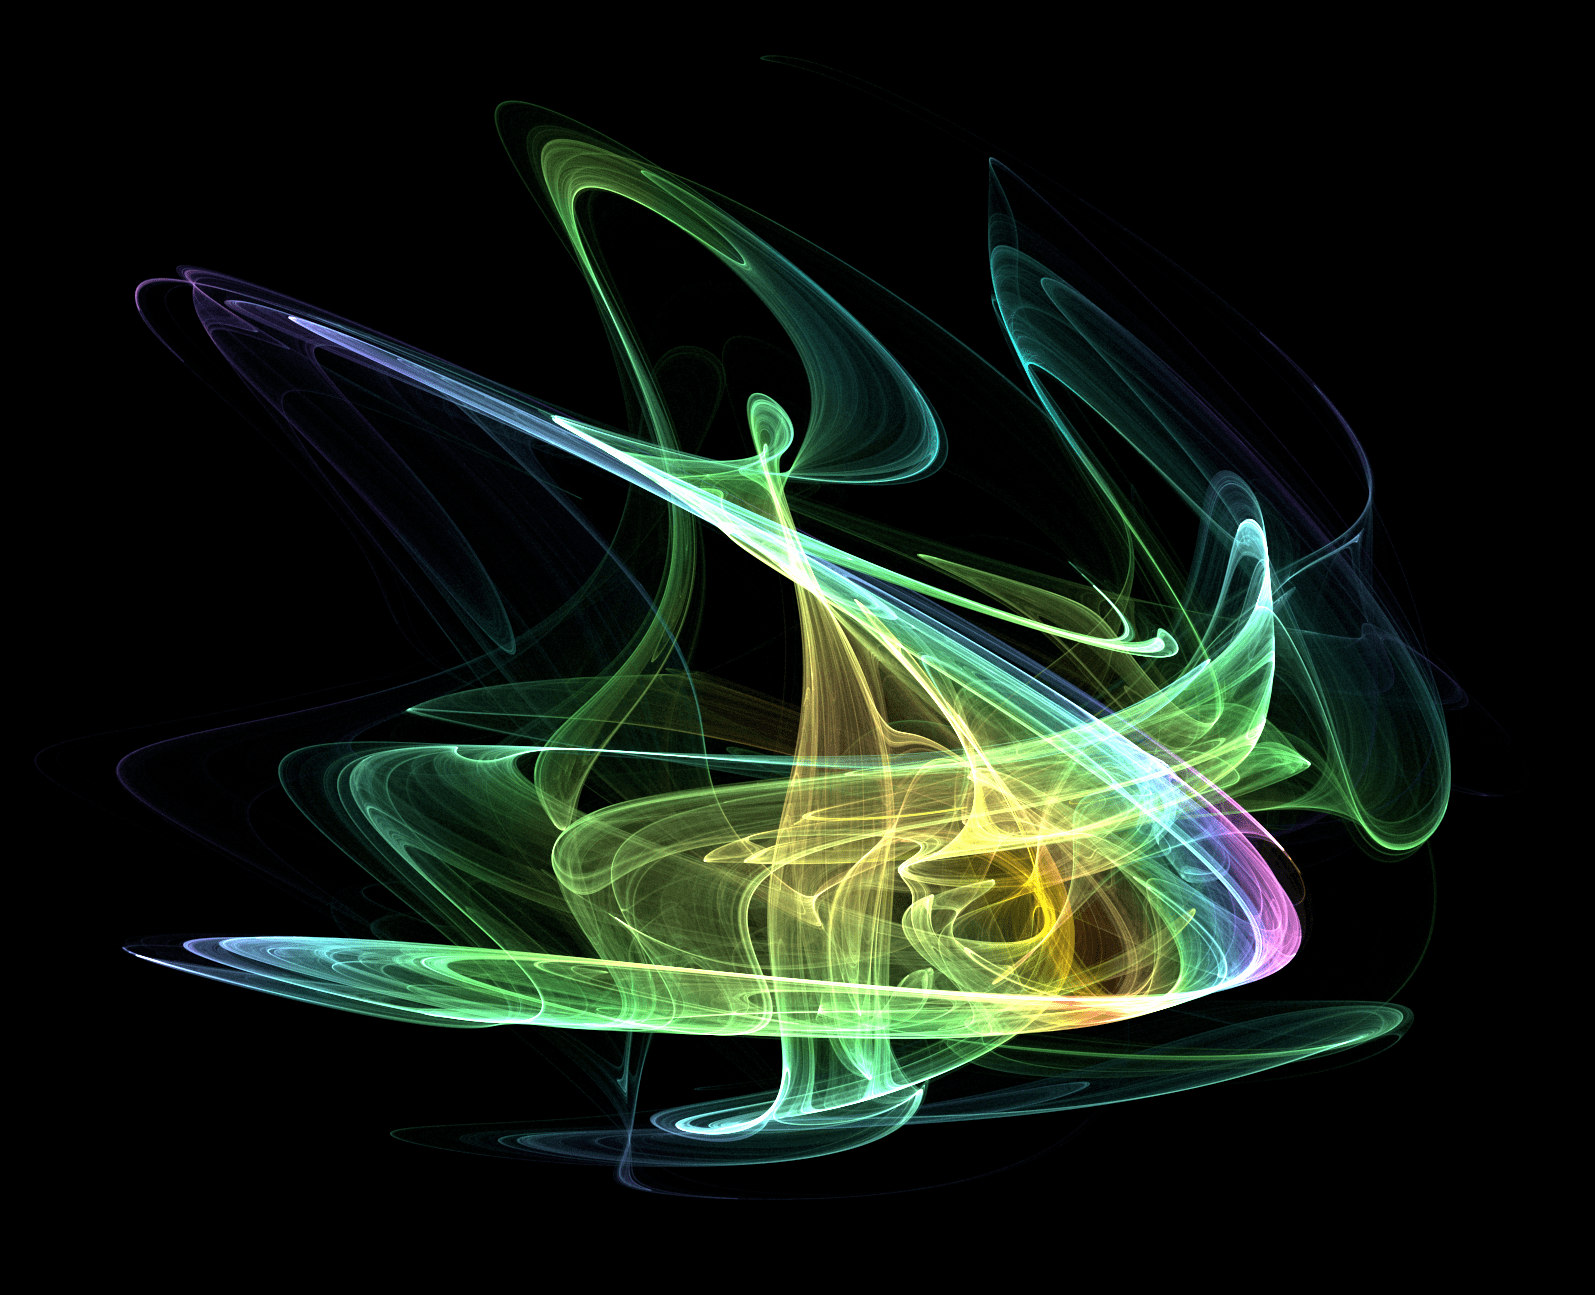
\includegraphics[height=3.2cm,width=3.7cm]{chaos/compressed/target_light.png}
		\caption{Ground truth}
	\end{subfigure}
	\caption{A series of trajectories for different parameters, demonstrating convergence to the true attractor.  The colormap is based on the speed and curvature of the trajectory, with rendering done using the program Chaoscope (available at {\href{http://www.chaoscope.org/}{http://www.chaoscope.org/}}). \label{fig:chaoscope}}
\end{figure}

Our first MMAP example considers the case of learning the dynamics parameters of a chaotic attractor.  
Specifically, we will aim to optimize the parameters of a Kalman smoother,
where we observe a noisy signal 
$y_t \in \real^{K}, \; t = 1,2,\dots,T$ in some $K$ dimensional observation space and each 
observation has a lower dimensional latent parameter $x_t \in \real^{D},  \; t = 1,2,\dots,T$.
In addition to an initial distribution $x_1 \sim \mathcal{N} \left(\mu_1, \sigma_1 I\right)$, our model is specified by 
\begin{subequations}
	\label{eq:Kalman}
\begin{align}
x_t = & A \left(x_{t-1}, \theta\right)+\delta_{t-1}, \; & \delta_{t-1} \sim \mathcal{N} \left(0, \sigma_q I\right) \\
y_t = & C x_{t}+\varepsilon_{t}, \; & \varepsilon_{t} \sim \mathcal{N} \left(0, \sigma_y I\right)
\end{align}
\end{subequations}
where $I$ is the identity matrix, $C$ is a known $K \times D$ matrix, and $\mu_1,\sigma_1, \sigma_q$ 
and $\sigma_y$ are all known scalars.  Our aim is to learn the dynamics parameters $\theta$ given
$y_{1:T}$, marginalizing over the latent variables $x_{1:T}$.  We use
a uniform prior on the parameters $\theta$, which means that the MMAP values for $\theta$
coincide with their (constrained) MML values.  A synthetic dataset was generated with $T=500$ and
$K=20$ (see \cite{rainforth2017boppArxiv}).
Inference on \qmarg was carried out using SMC with 500 particles.  
Convergence results are given in Figure~\ref{fig:chaos} showing that BOPP comfortably 
outperforms the PMMH variants, while Figure~\ref{fig:chaoscope} shows the simulated 
attractors generated from the dynamics parameters output by various iterations of a 
particular run of BOPP.
